% Lines starting with a percent sign (%) are comments. LaTeX will 
% not process those lines. Similarly, everything after a percent 
% sign in a line is considered a comment. To produce a percent sign
% in the output, write \% (backslash followed by the percent sign). 
% ==================================================================
% Usage instructions:
% ------------------------------------------------------------------
% The file is heavily commented so that you know what the various
% commands do. Feel free to remove any comments you don't need from
% your own copy. When redistributing the example thesis file, please
% retain all the comments for the benefit of other thesis writers! 
% ==================================================================
% Compilation instructions: 
% ------------------------------------------------------------------
% Use pdflatex to compile! Input images are expected as PDF files.
% Example compilation:
% ------------------------------------------------------------------
% > pdflatex thesis-example.tex
% > bibtex thesis-example
% > pdflatex thesis-example.tex
% > pdflatex thesis-example.tex
% ------------------------------------------------------------------
% You need to run pdflatex multiple times so that all the cross-references
% are fixed. pdflatex will tell you if you need to re-run it (a warning
% will be issued)  
% ------------------------------------------------------------------
% Compilation has been tested to work in ukk.cs.hut.fi and kosh.hut.fi
% - if you have problems of missing .sty -files, then the local LaTeX
% environment does not have all the required packages installed.
% For example, when compiling in vipunen.hut.fi, you get an error that
% tikz.sty is missing - in this case you must either compile somewhere
% else, or you cannot use TikZ graphics in your thesis and must therefore
% remove or comment out the tikz package and all the tikz definitions. 
% ------------------------------------------------------------------

% Document class for the thesis is report
% ------------------------------------------------------------------
% You can change this but do so at your own risk - it may break other things.
% Note that the option pdftext is used for pdflatex; there is no
% pdflatex option. 
% ------------------------------------------------------------------
\documentclass[12pt,a4paper,oneside,pdftex]{report}

% The input files (tex files) are encoded with the latin-1 encoding 
% (ISO-8859-1 works). Change the latin1-option if you use UTF8 
% (at some point LaTeX did not work with UTF8, but I'm not sure
% what the current situation is) 
\usepackage[latin1]{inputenc}
% OT1 font encoding seems to work better than T1. Check the rendered
% PDF file to see if the fonts are encoded properly as vectors (instead
% of rendered bitmaps). You can do this by zooming very close to any letter 
% - if the letter is shown pixelated, you should change this setting 
% (try commenting out the entire line, for example).  
\usepackage[OT1]{fontenc}
% The babel package provides hyphenating instructions for LaTeX. Give
% the languages you wish to use in your thesis as options to the babel
% package (as shown below). You can remove any language you are not
% going to use.
% Examples of valid language codes: english (or USenglish), british, 
% finnish, swedish; and so on.
\usepackage[finnish,english]{babel}


% Optional packages
% ------------------------------------------------------------------
% Select those packages that you need for your thesis. You may delete
% or comment the rest.

% Natbib allows you to select the format of the bibliography references.
% The first example uses numbered citations: 
\usepackage[square,sort&compress,numbers]{natbib}
% The second example uses author-year citations.
% If you use author-year citations, change the bibliography style (below); 
% acm style does not work with author-year citations.
% Also, you should use~\citet (cite in text) when you wish to refer
% to the author directly (\citet{blaablaa} said blaa blaa), and 
%~\citep when you wish to refer similarly than with numbered citations
% (It has been said that blaa blaa~\citep{blaablaa}).
% \usepackage[square]{natbib}

% The alltt package provides an all-teletype environment that acts
% like verbatim but you can use LaTeX commands in it. Uncomment if 
% you want to use this environment. 
% \usepackage{alltt}

% The eurosym package provides a euro symbol. Use with \euro{}
\usepackage{eurosym} 

% Verbatim provides a standard teletype environment that renderes
% the text exactly as written in the tex file. Useful for code
% snippets (although you can also use the listings package to get
% automatic code formatting). 
\usepackage{verbatim}

% The listing package provides automatic code formatting utilities
% so that you can copy-paste code examples and have them rendered
% nicely. See the package documentation for details.
% \usepackage{listings}

% The fancuvrb package provides fancier verbatim environments 
% (you can, for example, put borders around the verbatim text area
% and so on). See package for details.
% \usepackage{fancyvrb}

% Supertabular provides a tabular environment that can span multiple 
% pages. 
%\usepackage{supertabular}
% Longtable provides a tabular environment that can span multiple 
% pages. This is used in the example acronyms file. 
\usepackage{longtable}

% The fancyhdr package allows you to set your the page headers 
% manually, and allows you to add separator lines and so on. 
% Check the package documentation. 
% \usepackage{fancyhdr}

% Subfigure package allows you to use subfigures (i.e. many subfigures
% within one figure environment). These can have different labels and
% they are numbered automatically. Check the package documentation. 
\usepackage{subfigure}

% The titlesec package can be used to alter the look of the titles 
% of sections, chapters, and so on. This example uses the ``medium'' 
% package option which sets the titles to a medium size, making them
% a bit smaller than what is the default. You can fine-tune the 
% title fonts and sizes by using the package options. See the package
% documentation.
\usepackage[medium]{titlesec}

% The TikZ package allows you to create professional technical figures.
% The learning curve is quite steep, but it is definitely worth it if 
% you wish to have really good-looking technical figures. 
\usepackage{tikz}
% You also need to specify which TikZ libraries you use
\usetikzlibrary{positioning}
\usetikzlibrary{calc}
\usetikzlibrary{arrows}
\usetikzlibrary{decorations.pathmorphing,decorations.markings}
\usetikzlibrary{shapes}
\usetikzlibrary{patterns}


% The aalto-thesis package provides typesetting instructions for the
% standard master's thesis parts (abstracts, front page, and so on)
% Load this package second-to-last, just before the hyperref package.
% Options that you can use: 
%   mydraft - renders the thesis in draft mode. 
%             Do not use for the final version. 
%   doublenumbering - [optional] number the first pages of the thesis
%                     with roman numerals (i, ii, iii, ...); and start
%                     arabic numbering (1, 2, 3, ...) only on the 
%                     first page of the first chapter
%   twoinstructors  - changes the title of instructors to plural form
%   twosupervisors  - changes the title of supervisors to plural form
% \usepackage[mydraft]{aalto-thesis}
\usepackage[mydraft,doublenumbering]{aalto-thesis}
%\usepackage{aalto-thesis}


% Hyperref
% ------------------------------------------------------------------
% Hyperref creates links from URLs, for references, and creates a
% TOC in the PDF file.
% This package must be the last one you include, because it has
% compatibility issues with many other packages and it fixes
% those issues when it is loaded.   
\RequirePackage[pdftex]{hyperref}
% Setup hyperref so that links are clickable but do not look 
% different
\hypersetup{colorlinks=false,raiselinks=false,breaklinks=true}
\hypersetup{pdfborder={0 0 0}}
\hypersetup{bookmarksnumbered=true}
% The following line suggests the PDF reader that it should show the 
% first level of bookmarks opened in the hierarchical bookmark view. 
\hypersetup{bookmarksopen=true,bookmarksopenlevel=1}
% Hyperref can also set up the PDF metadata fields. These are
% set a bit later on, after the thesis setup.   


% Thesis setup
% ==================================================================
% Change these to fit your own thesis.
% \COMMAND always refers to the English version;
% \FCOMMAND refers to the Finnish version; and
% \SCOMMAND refers to the Swedish version.
% You may comment/remove those language variants that you do not use
% (but then you must not include the abstracts for that language)
% ------------------------------------------------------------------
% If you do not find the command for a text that is shown in the cover page or
% in the abstract texts, check the aalto-thesis.sty file and locate the text
% from there. 
% All the texts are configured in language-specific blocks (lots of commands
% that look like this: \renewcommand{\ATCITY}{Espoo}.
% You can just fix the texts there. Just remember to check all the language
% variants you use (they are all there in the same place). 
% ------------------------------------------------------------------
\newcommand{\TITLE}{Privacy Implications of WLAN Probing}
\newcommand{\FTITLE}{Yksityisyydensuoja langattomissa verkoissa}
\newcommand{\SUBTITLE}{}
\newcommand{\FSUBTITLE}{}
\newcommand{\DATE}{August 5, 2014}
\newcommand{\FDATE}{5. elokuuta 2014}

% Supervisors and instructors
% ------------------------------------------------------------------
% If you have two supervisors, write both names here, separate them with a 
% double-backslash
% Also remember to add the package option ``twosupervisors'' or
% ``twoinstructors'' to the aalto-thesis package so that the titles are in
% plural.

\newcommand{\SUPERVISOR}{Professor Tuomas Aura}
\newcommand{\FSUPERVISOR}{Professori Tuomas Aura}

\newcommand{\INSTRUCTOR}{Professor Christopher Kruegel}
\newcommand{\FINSTRUCTOR}{Professori Christopher Kruegel}

\newcommand{\COVERSUPERVISOR}{Professor Tuomas Aura, Aalto University}
\newcommand{\COVERINSTRUCTOR}{Professor Christopher Kruegel, University of California, Santa Barbara}


% Other stuff
% ------------------------------------------------------------------
\newcommand{\PROFESSORSHIP}{Data Communication Software}
\newcommand{\FPROFESSORSHIP}{Tietoliikenneohjelmistot}

% Professorship code is the same in all languages
\newcommand{\PROFCODE}{T-110}
\newcommand{\KEYWORDS}{}
\newcommand{\FKEYWORDS}{}

\newcommand{\LANGUAGE}{English}
\newcommand{\FLANGUAGE}{Englanti}

% Author is the same for all languages
\newcommand{\AUTHOR}{Pekko Lipsanen}


% Currently the English versions are used for the PDF file metadata
% Set the PDF title
\hypersetup{pdftitle={\TITLE\ \SUBTITLE}}
% Set the PDF author
\hypersetup{pdfauthor={\AUTHOR}}
% Set the PDF keywords
\hypersetup{pdfkeywords={\KEYWORDS}}
% Set the PDF subject
\hypersetup{pdfsubject={Master's Thesis}}


% Layout settings
% ------------------------------------------------------------------

% Use this to control how much space there is between each line of text.
% 1 is normal (no extra space), 1.3 is about one-half more space, and
% 1.6 is about double line spacing.  
% \linespread{1} % This is the default
% \linespread{1.3}

% Bibliography style
% acm style gives you a basic reference style. It works only with numbered
% references.
\bibliographystyle{acm}
% Plainnat is a plain style that works with both numbered and name citations.
% \bibliographystyle{plainnat}


% Extra hyphenation settings
% ------------------------------------------------------------------
% You can list here all the files that are not hyphenated correctly.
% You can provide many \hyphenation commands and/or separate each word
% with a space inside a single command. Put hyphens in the places where
% a word can be hyphenated.
% Note that (by default) LaTeX will not hyphenate words that already
% have a hyphen in them (for example, if you write ``structure-modification 
% operation'', the word structure-modification will never be hyphenated).
% You need a special package to hyphenate those words.
% \hyphenation{di-gi-taa-li-sta yksi-suun-tai-sta}


% The preamble ends here, and the document begins. 
% Place all formatting commands and such before this line.
% ------------------------------------------------------------------
\begin{document}
% This command adds a PDF bookmark to the cover page. You may leave
% it out if you don't like it...
\pdfbookmark[0]{Cover page}{bookmark.0.cover}
% This command is defined in aalto-thesis.sty. It controls the page 
% numbering based on whether the doublenumbering option is specified
\startcoverpage

% Cover page
% ------------------------------------------------------------------
% Options: finnish, english, and swedish
% These control in which language the cover-page information is shown
\coverpage{english}


% Abstracts
% ------------------------------------------------------------------
% Include an abstract in the language that the thesis is written in,
% and if your native language is Finnish or Swedish, one in that language.

% Abstract in English
% ------------------------------------------------------------------
\thesisabstract{english}{

}

% Abstract in Finnish
% ------------------------------------------------------------------
\thesisabstract{finnish}{

}

% Acknowledgements
% ------------------------------------------------------------------
% Select the language you use in your acknowledgements
\selectlanguage{english}

% Uncomment this line if you wish acknoledgements to appear in the 
% table of contents
%\addcontentsline{toc}{chapter}{Acknowledgements}

% The star means that the chapter isn't numbered and does not 
% show up in the TOC
\chapter*{Acknowledgements}

I wish to thank all students who use \LaTeX\ for formatting their theses,
because theses formatted with \LaTeX\ are just so nice.

Thank you, and keep up the good work!
\vskip 10mm

\noindent Espoo, \DATE
\vskip 5mm
\noindent\AUTHOR

% Acronyms
% ------------------------------------------------------------------
% Use \cleardoublepage so that IF two-sided printing is used 
% (which is not often for masters theses), then the pages will still
% start correctly on the right-hand side.
\cleardoublepage
% Example acronyms are placed in a separate file, acronyms.tex
\addcontentsline{toc}{chapter}{Abbreviations and Acronyms}
\chapter*{Abbreviations and Acronyms}

% The longtable environment should break the table properly to multiple pages, 
% if needed

\noindent
\begin{longtable}{@{}p{0.25\textwidth}p{0.7\textwidth}@{}}
BSSID & Basic Service Set Identifier \\
CCTV & Closed Circuit Television \\
EU & European Union \\
ESS & Extended Service Set \\
ESSID & Extended Service Set Identifier \\
HT & High throughput \\
IEEE & Institute of Electrical and Electronics Engineers \\
JSON & JavaScript Object Notation \\
MAC & Media Access Control \\
MCL & Markov Cluster \\
MITM & Man in the middle \\
QoS & Quality of Service \\
SSID & Service Set Identifier \\
SSL & Secure Sockets Layer \\
TLS & Transport Layer Security \\
UUID & Universally Unique Identifier \\
WLAN & Wireless Local Area Network \\
WPA & Wi-Fi Protected Access \\
WPS & Wi-Fi Protected Setup \\
\end{longtable}


% Table of contents
% ------------------------------------------------------------------
\cleardoublepage
% This command adds a PDF bookmark that links to the contents.
% You can use \addcontentsline{} as well, but that also adds contents
% entry to the table of contents, which is kind of redundant.
% The text ``Contents'' is shown in the PDF bookmark. 
\pdfbookmark[0]{Contents}{bookmark.0.contents}
\tableofcontents

% List of tables
% ------------------------------------------------------------------
% You only need a list of tables for your thesis if you have very 
% many tables. If you do, uncomment the following two lines.
% \cleardoublepage
% \listoftables

% Table of figures
% ------------------------------------------------------------------
% You only need a list of figures for your thesis if you have very 
% many figures. If you do, uncomment the following two lines.
% \cleardoublepage
% \listoffigures

% The following label is used for counting the prelude pages
\label{pages-prelude}
\cleardoublepage

%%%%%%%%%%%%%%%%% The main content starts here %%%%%%%%%%%%%%%%%%%%%
% ------------------------------------------------------------------
% This command is defined in aalto-thesis.sty. It controls the page 
% numbering based on whether the doublenumbering option is specified
\startfirstchapter

% Add headings to pages (the chapter title is shown)
\pagestyle{headings}


%%%%%%%%%%%%%%%%%%%%%%%%%%%%%%%%%%%%%%%%%%%%%%%%%%%%%%%%%%%%%%%%%%%%%%%%%%%%%%%


\chapter{Introduction}
\label{chapter:intro}

Wireless technology has been established well in everyday life. Most of people have nowadays their own wireless network at home and they use another at school or work. When traveling, hotels and airports almost always offer Wi-Fis, in many cases for free. Wireless networks can also be found in shopping malls, even in buses and trains -- and the number of networks is only growing.

From the very nature of wireless networks, transferred data is always visible to everyone who is inside the range of the network. Compared to traditional on-wire networking, this creates worries for information security. Lots of work has been done in order to make sure that actual transferred data, for example the content of web pages browsed, remains confident and is not visible for eavesdroppers. Such work include, for example, standards for wireless network encryption.

However, we are interested in the data exchange that happens before a device joins a wireless network. The device has not established any connections yet, so all the information must be sent in plaintext, unencrypted, in public. This information includes at least the identifier of the device trying to connect to the network, and the network name it is trying to connect. Or, alternatively, the device can ask information about all networks in the range.

% Say something about always-on scanning?

In this thesis, we try to examine what information can be extracted for said part of data transmission, and how it can be used. For this part, we conduct a practical experiment. We will also examine legal position of doing so, and are not limited to techincal part of the issue. In addition, we will look for techincal countermeasures for found privacy threats: how our techniques can be circumvented, if wanted.

The thesis is organized as follows. In Chapter~\ref{chapter:protocol}, we tell how the 802.11 protocol, also known as Wi-Fi, works. In Chapter~\ref{chapter:profiling} we will examine how and why parts of wireless network protocols can be used for tracking and profiling users. We will also briefly study the legal side of tracking and profiling. Further, in Chapter~\ref{chapter:attacks} we will see how these features can be used in conducting active attacks and not only passive monitoring of devices. Practical experiment of above-mentioned techniques is conducted in Chapter~\ref{chapter:practical}, and in Chapter~\ref{chapter:countermeasures} we will see how privacy-concerned users could be protected from the actions we have studied. Finally, in Chapter~\ref{chapter:conclusion} we conclude the thesis.


%%%%%%%%%%%%%%%%%%%%%%%%%%%%%%%%%%%%%%%%%%%%%%%%%%%%%%%%%%%%%%%%%%%%%%%%%%%%%%%


\chapter{The 802.11 wireless network protocol}
\label{chapter:protocol}


\section{Introductory to wireless networks}
\label{sec:intro_wireless}

Wireless connections can be divided into two categories. First, we have cell-based technologies, which are used between mobile network operator (such as Verizon, T-Mobile) and a mobile device. Such technologies include but are not limited to GPRS, EDGE, and UMTS. This thesis does not study these protocols.

We will examine the protocols and data transmissions used inside local area networks (LAN). Traditionally, those networks have been made connecting cables between computers and a hub, a switch or a router. Recently these local networks have been built with wireless connections, as they obviously allow users great mobility. Also, as smartphones have developed and require more and more bandwidth, local area networks are easier and cheaper to build and used than mobile networks.

The protocol for wireless LAN (WLAN) is maintained the IEEE LAN/MAN Standards Committee, also known as IEEE 802. The family of protocols covering WLAN is called 802.11 family, and it includes many different versions of the standard, denoted by letters. For example, widely implemented standards are 802.11b, 802.11g, and 802.11n.~\cite{IEEE802.11}


\section{Wireless networks terminolgy}
\label{sec:terminology}

Inside a wireless network there can be found several different devices. In the following, we will put them into different categories.

IEEE, a standards organization maintaining the wireless standard, defines all the devices capable to connect wireless network as \emph{stations} (STA). However, this definition is a bit too broad, so we will split it further.

First there can be found devices only connecting to network, which we will call \emph{nodes}. A node can be any kind of device, and most common and most relevant ones for this study are laptops and smartphones. 

Second, the devices building the wireless network and allowing nodes to connect to it are called \emph{Access points} (AP). A wireless network can consist of one or more APs.

Access points and nodes associated with it form a network, which can also be called \emph{Basic Service Set} (BSS). In this thesis, we refer to that simply as \emph{wireless network} or shortly as \emph{network}, if there is no room for confusion.

Nodes can also work in \emph{ad-hoc} mode, where they act simultaneously as an access point and as a node without well-defined structure. However, these networks are not common, and we will not cover them in this thesis.


\section{MAC Address}
\label{sec:MAC}

Every device in the network, wired and wireless, has a media access control (MAC) address. A MAC address is bound to a specific device and does not change while connecting to different networks, being reconfigured, restarted, or anything else. It should also be globally unique: the idea is that any two devices could join the same network without problems, and since the network needs to be able to differentiate between devices, every device must have a unique identifier.~\cite{802_overview}

A MAC address is 48 bit long and consists of two independent 24-bit parts. The first part is the same for all the devices made by the same manufacturer, and that part is assigned by IEEE. This first part is called Organizationally Unique Identifier, or OUI. 

The second 24-bit part can be freely chosen by the manufacturer, but it should be unique for each device. 

The real address space of OUI, the organization part of address, is 22 bits, because one of the 24 bits (the least significant) depends on application, and another (next to LSB) is always set zero. Therefore there is space for $2^{22}$ organizations, which is a bit over four million. Each organization can produce $2^{24}$ devices, which is more than 16 million. If this limit is exceeded, IEEE can give the organization another OUI. For example, Apple has more than 300 OUIs assigned.~\cite{oui_listing} However, IEEE states that it will not do so without proper reasons, and says that, ``in no way should these addresses be used for purposes that would lead to skipping large numbers of them''.~\cite{802_overview} 

MAC addresses are presented in hexadecimal notation consisting of six octects, seperated by a colon or a dash, for example \texttt{54:26:96:d0:2c:b1}. Graphical representation of a MAC address is shown in Figure~\ref{fig:mac}, where the first row is a raw binary representation, and the second row shows hexadecimal values. The last row shows seperation between Organizationally Unique Identifier and the part that remains to be determined by the manufacturer.

\begin{figure}
\label{fig:mac}
\begin{tabular}{ | c|c|c | c|c|c | }
  \hline
  1010100 & 100110 & 10010110 & 11010000 & 101100 & 10110001 \\
  \hline
  54 & 26 & 96 & d0 & 2c & b1 \\
  \hline
  \multicolumn{3}{|c|}{Organizationally Unique Identifier} & \multicolumn{3}{c|}{Organization-controlled part} \\
  \hline
\end{tabular}
\caption{Strucutre of MAC address \texttt{54:26:96:d0:2c:b1}}
\end{figure}


\section{Service Set Identifier (SSID)}
\label{sec:SSID}

As we found in the last section, each device in a network has a unique identifier, a MAC address. If there are multiple APs available for a node to connect to, the node can recognize and select the one by AP's MAC address.

However, such action usually requires human interaction: someone has to tell the node which one of the APs is the correct one. Using only MAC address is not convinient, since twelwe-character hexadecimal representation does not resemble anything familiar or memorizable.

Also, physical network devices do not necessarily correspond to logical networks. There can be a wireless network in a university, where APs are being upgraded to new ones. Therefore the logical network is still the same in the same building with the same purpose, but all the MAC addresses of the APs have been changed: remember, every MAC address is globally unique.

To solve the problem, there is a concept of SSID, \emph{Service Set Identifier}. APs are given a human-readable string, the SSID, which has maximum length of 32 characters. This can be thought as a name of the network.

With SSID there is an abstraction of logical network over a physical one. Using the same example as before, if the university's wireless network keeps the same SSID, its APs can be updated without any problems: nodes will still find the correct network, even if the hardware is completely different and MAC addresses do not match anymore.

Network can also consist of more than one APs sharing the same SSID. This way, a wireless network can cover a huge building or even a larger area. When configured in such way, the network is said to be an \emph{Extended Service Set} (ESS).~\cite{IEEE802.11}


\section{Joining a network}
\label{sec:joining}

So far we have characterized different elements of a wireless network. In this section, we will discuss how a node can find a existing wireless network. This can be achieved using either (1) active scanning or (2) passive scanning, which both are defined in IEEE standard.~\cite{IEEE802.11_scanning}

\subsection{Passive scanning}
\label{subsec:passive_scanning}

In passive scanning, a node does not send anything by itself in order to find the network it wants to join. Instead, a node listens the transmissions and scans for beacon frames sent by APs. Beacon frames are large and contain lots of information, total of 55 different fields, most of which are related to radio transmission parameters.

However, while doing passive scanning, a node is only interested in one particular field, SSID. As we have learnt previously in Section~\ref{sec:SSID}, SSID identifies particular network and acts as a human-understandable network name. Therefore node can display the networks it found to end-user, who makes the decision which network to join. Alternatively, node can compare its findings to previously-generated list of known networks, and join one it finds interesting.

Passive scanning has some drawbacks. First, it might be relatively slow, as a node needs to wait for APs to broadcast their beacons. Secondly, it is possible to configure AP so that it does not broadcast its SSID: this feature is called \emph{Hidden SSID}. Therefore, a node using passive scanning never sees APs using Hidden SSIDs.

\subsection{Active scanning}
\label{subsec:active_scanning}

In active scanning, the situation is different. This time a node knows beforehand which network it would like to join, and sends \emph{probe request frames} into the air. 

Probe requests are smaller than previously-mentioned beacon frames, having only 13 standard fields. The most important field for our study is the first one, SSID. In this field a node tells which network it would like to join, if possible. 

If a node knows lots of different networks and is trying to join all of them, it needs to send a lot of probe request frames. In order to reduce the amount of network traffic, there is a field called ``SSID List'', 10th in probe request frame. Using this field, a node can combine several requests into a single one. The length of the list is variable, and is limited only by the fact that the actual ``length'' field of SSID List element has size of one octet. Therefore the maximum number of SSIDs in a single SSID List element is 256.

\subsection{Active scanning with a wildcard SSID}
\label{subsec:active_wildcard}

There exists also a combination of active and passive scanning. A node can request information of all present wireless networks by sending a probe request frame with wildcard SSID. This way, the node does not state which networks it knows or want to join, but it also does not need to wait APs to advertise themselves by beacon frames.

IEEE Standard states wildcard SSID to be the one with all bits set to zero. 


%%%%%%%%%%%%%%%%%%%%%%%%%%%%%%%%%%%%%%%%%%%%%%%%%%%%%%%%%%%%%%%%%%%%%%%%%%%%%%%


\chapter{Profiling and tracking}
\label{chapter:profiling}

\section{Customer profiling and tracking}
\label{sec:profiling}

Before beginning, we will define what profiling means. First, Oxford English dictionary defines the term as:~\cite{oed_profiling}

\begin{quotation}
The recording, itemization, or analysis of a person's known psychological, intellectual, and behavioural characteristics, esp. as documentation used (in schools, businesses, etc.) in the assessment of an individual's capabilities; (also) the compilation of databases which store such information and that can be used to identify any particular subgroup of people.
\end{quotation}

A little more relevant definition for this study could be one written by Hilberdant:~\cite{hildebrandt2008}

\begin{quotation}
The process of ``discovering'' correlations between data in databases that can be used to identify and represent a human or nonhuman subject (individual or group), and/or the application of profiles (sets of correlated data) to individuate and represent a subject or to identify a subject as a member of a group or category.
\end{quotation}

In this thesis, we are interestered in profiling in a sense of discovering some charasteristics of a person from collected data. As mentioned in both of definitions above, we are not limited to profiling single persons, but may also look for particular groups of people, if they have interesting properties in common.

For example, it might be useful to know how old the customers are on average or if they are interested in different product ranges or visit a store different times of a day. An interesting - yet difficult to provide - property would be customer's wealth or willingess to pay more. If seller could detect these kind of people, it could easily gain its revenue by promoting more expensive deals to these kind of people.

\textbf{Tracking} is easier to define. We use it to mean situation where one follows another person's movements or actions, directly or by following a device owned by tracked person. 

Tracking and profiling in themselves do not produce any value. However, information generated by them can be used to design new marketing campaigns and strategies, adjust prices, or otherwise promote sales.

An example of price variation based on customer profiling can be found in experiment made by Deck and Wilson (2006)~\cite{Deck2006}. In the research, they divided customers into two categories based on their search history. The first group is called ``informed customers'', who have been searching for prices also from other stores. On the other hand, the second group of users is called ``uninformed'', who do not know about the general prices of a product. The results of experiment shows that with tracking, informed customers are given lower prices, whereas ignorance of uninformed customers can be exploited with higher prices.

On internet it is easy to profile users of a webpage. In a study by Pekkala et al.~\cite{Pakkala2012504} researchers try to analyze what kind of people are using food composition websites in three different countries. They used Google Analytics~\cite{googleanalytics}, a free and available-to-everyone tool to gather visitor statistics (also other similiar tools are available, with or without a charge). By looking referential websites, usage patterns, and search terms they were able to conduct that, for example, most of the users were not food or nutrition professionals, but average people looking for basic information about nutrition. In the study, researchers conclude that ``web analytics should be routine for every website [..] making user behaviour clearer so that developers can produce better websites for users.''

For the physical, brick-and-mortar type of stores, achieving this kind of information is much more diffcult. They can conduct customer studies by using surveys, but such a study requires lots of resources and might not be trustworthy because of reponse bias~\cite{Furnham1986385}: it may be totally different what people say than how they really act. Also, where it is extremely easy to track all the actions customers take while shopping on an online store, gathering the same data in traditional store using traditional methods can be close to impossible. Therefore it is easy to see that online stores have a clear competitive advantage over brick-and-mortar ones -- and the latters are interested in to neglect that.

Some solutions before establishment of WLAN devices have been proposed. An interesting one is work done by Newman, Yu and Oulton (2002) in~\cite{Newman2002253}, where they use existing CCTV surveillance cameras in a store. An example of their system is presented on Picture~\ref{fig:cctv_tracking}. Same kind of work is done by Senior et al.~\cite{senior2007video}, and in recent years there have been commercial solutions available~\cite{retailcctv}.

\begin{figure}
    \label{fig:cctv_tracking}
    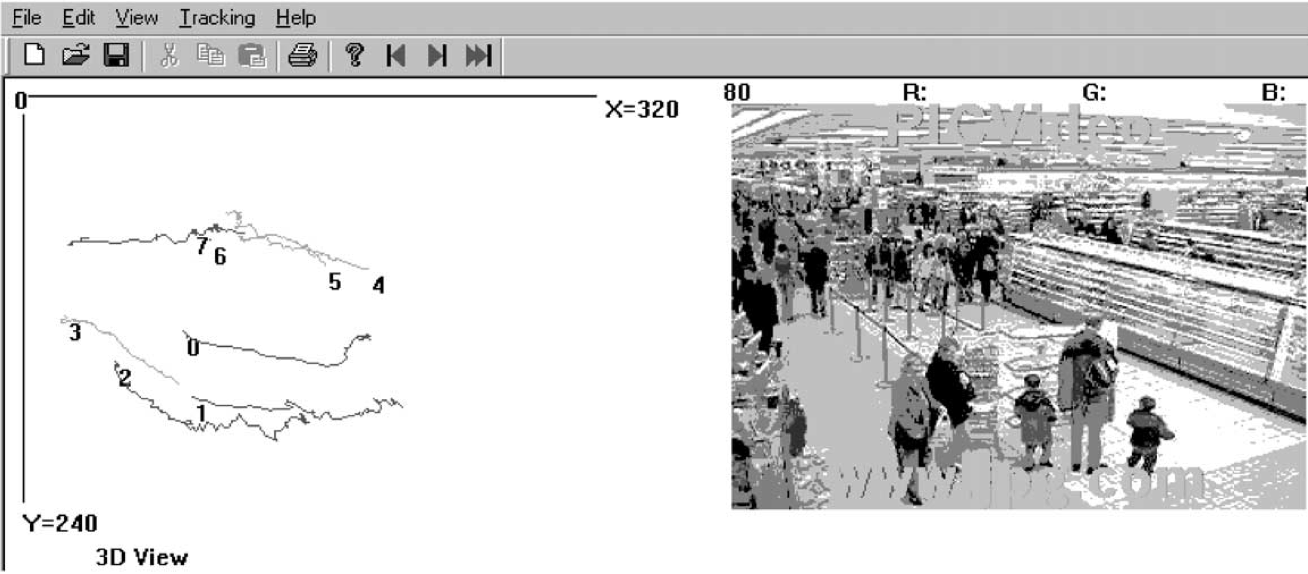
\includegraphics[width=\textwidth]{images/cctv_tracking_newman_pic1}
    \caption{Example of CCTV-based customer tracking from work by Newman et al~\cite{Newman2002253}}
\end{figure}


\section{Tracking using MAC address}
\label{sec:mac_tracking}

To see where a user has been and how he has moved, tracking system needs to be able to perform two operations. First, it needs to be able to determine the location of the device in question. Second, all the location data needs to be linked together, which means that a device needs to be assigned some form of a unique ID.

Wireless nodes send their MAC address with every probe request, as we learnt in Section~\ref{subsec:active_scanning}. This is also globally unique; see Section~\ref{sec:MAC}. MAC address seems to be a good candidate for an ID, so we can continue for a much harder problem, locating nodes.

\subsection{Determining the location of a node}
\label{sec:location}

A naive yet robust way to determine user's location would be to look which AP received node's probe request. In Picture~\ref{fig:position_1} an oversimplified situation is presented: there is a rectangular-shaped building with a room, a few shelves, and four access points, labeled with letters from A to D. The building is divided into four sections, and the position of a mobile device is determined by looking which AP received a request from it. For example, it might be assumed that only AP D recieves a signal from the mobile device in the picture, and therefore the user is somewhere in the lower-right section of the building.

\begin{figure}
    \label{fig:position_1}
    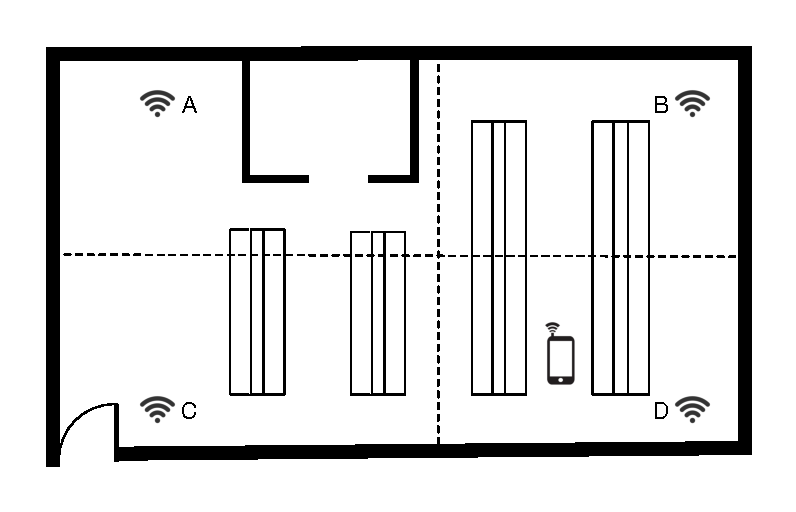
\includegraphics{images/positioning_1.pdf}
    \caption{Simplest way to achieve positioning}
\end{figure}

However, things are obviously not that simple. In real-life situations, coverage of a single AP can be large and easily overlap with others, and signal from the mobile device in Picture~\ref{fig:position_1} could also be in the ranges of APs B and C. A real-life example from~\cite{xiang2004} is presented in Picture~\ref{fig:ibm_coverage}, where in Figure~\ref{subfig:ibm_layout} the layout of building is presented, and in Figure~\ref{subfig:ibm_strength} the strength of a signal from a single AP is shown. Note that the whole floor is covered by the AP at least in some amount, but there are still four more APs. This suggests that at least in this case, a device can always catch more than one signal.

\begin{figure}
\begin{center}
\subfigure[Layout of the building]{
  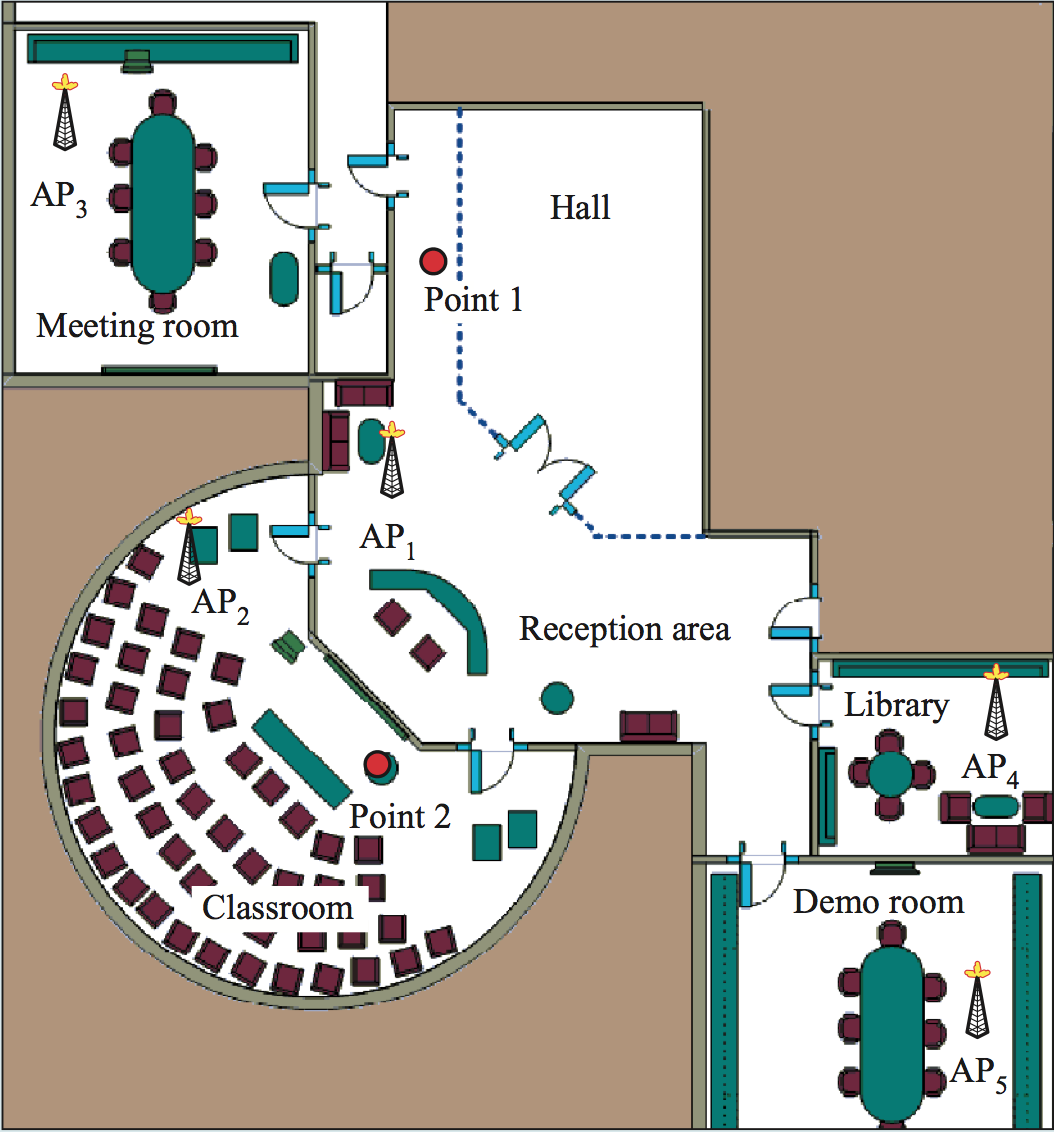
\includegraphics[scale=0.34]{images/ibm_wlan_layout.png}
  \label{subfig:ibm_layout}
}
\subfigure[Coverage of AP$_1$]{
  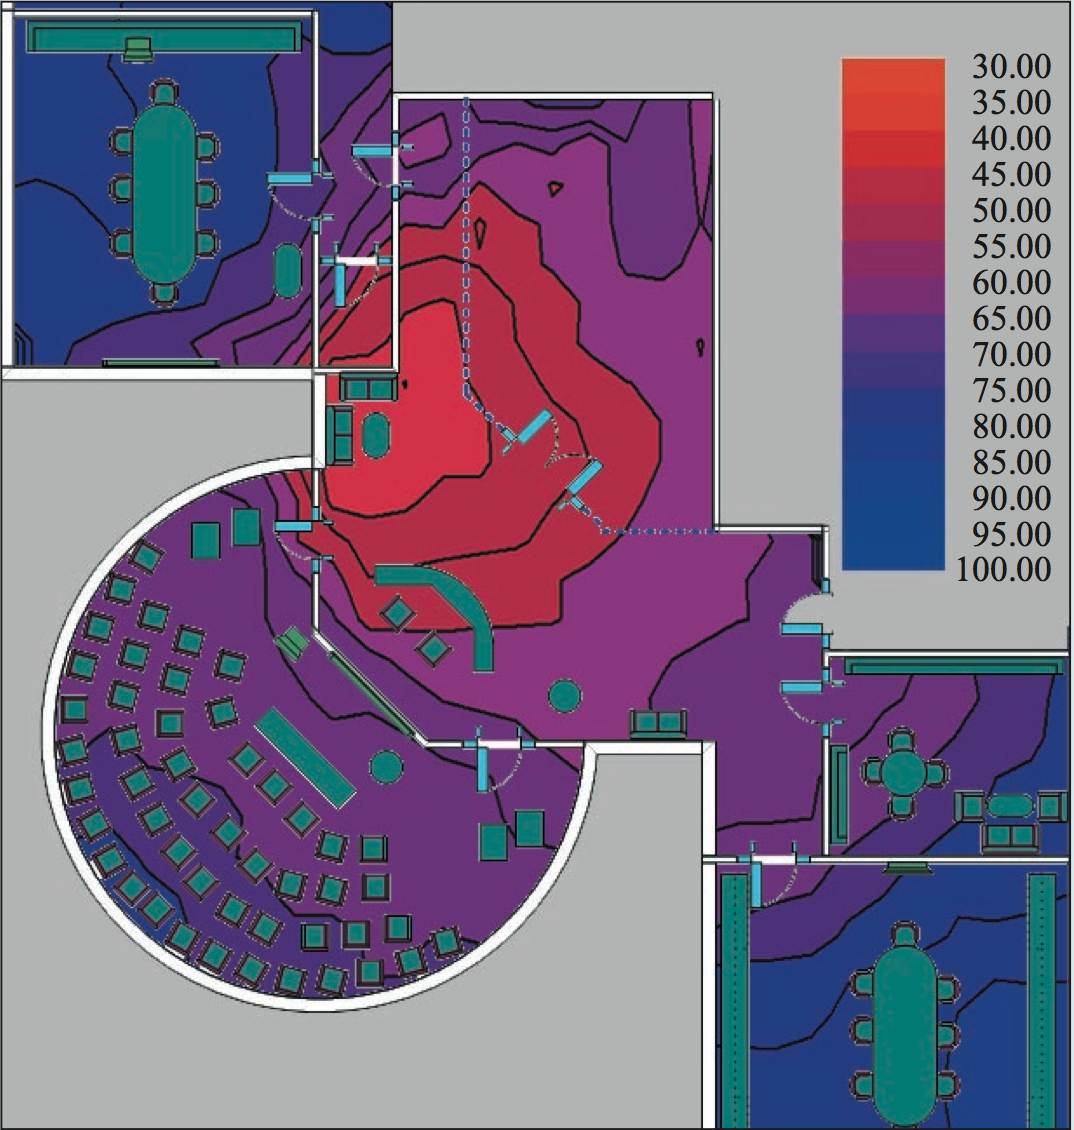
\includegraphics[scale=0.34]{images/ibm_wlan_strength.png}
  \label{subfig:ibm_strength}
}
\caption{A real-life example of WLAN coverage. Taken from~\cite{xiang2004}.}
\label{fig:ibm_coverage}
\end{center}
\end{figure}

Distance from a node to an AP can be estimated by using strength of radio signal. This can not give an exact distance, as transmitting power varies between devices, and we do not know the initial power. However, this problem does not prevent us from using it as an estimate, because we are interested in relative distances. Continuing the simple way, we can select an AP that recieved the strongest signal; for a little more accurate result, a triangular-based calculation could be done with simple trigonometry, if at least three APs received the signal.

Luckily, lots of research has been done for creating WLAN-based positioning systems, and that research includes more and more sophisticated methods for determining the location. Xiang et al.~\cite{xiang2004} constructed a model of signal propagation, Roos et al.~\cite{roos2002} used probablistics and machine learning, and so on. Most of this research tries to let mobile phone determine its own location based on the signal from APs, but exactly same approach can be used other way around, as we would like to: to let AP find out mobile node's position by node's signals.

--

track location inside a building; helsinki-vantaa airport, stores and shopping malls

\section{Profiling users using SSIDs from active scanning}
\label{sec:ssid_profiling}

Whereas previous section discussed on possibilities to track a device based on MAC address, in this chapter we will see how it is possible to profile users who have left active scanning running on their devices. Later we conduct a practical study based on techniques presented in this chapter; this is done in Chapter~\ref{chapter:practical}. 

\subsection{Geolocation}
\label{subsec:ssid_geo}

SSIDs do not necessarily leak any information about their location. In some cases the opposite may be true: for example, an open network in Aalto University is called ``Aalto open'', but in general no such connection can be drawn.

Numerous applications would benefit from ability to connect wirless network APs to physical geolocation. For example, this could serve as a backup solution in lack of GPS signal for positioning, which is the case when user is inside a building. Also it would be possible for mobile phone users to find a nearby open WLAN instead of consuming expensive cellular data transfer.

The solution for this problem is simple and straightforward. A collecting device goes around the world, capturing all the SSIDs and MAC addresses of WLANs it finds. Then, using GPS, it gets the location of network and stores data into simple database. This has already been done by numerous companies: the best-known case might be Google, who did it with its Street View cars~\cite{google_wifi_collection}. 

Another way to get the data is to use crowdsourcing -- in other words, to let users do it themselves. In this way, every time a user connects to a new network, exact geolocation is saved with phone's GPS receiver. The location, SSID of the network, and probably more information such as signal strength are then saved into a database. Using this approach, data-collecting company can gather lots of data relatively cheaply, and may be able to achieve higher accuracy compared to smaller dataset.

Both of above-explained applications for geolocation data of wireless networks have been implemented. Google uses WLAN locations with its Android operating system to provide location data based on networks it finds around~\cite{google_wifi_collection}. Nokia and Microsoft use same kind of data in Windows Phone in order to locate open WLANs near the user's own location~\cite{nokia_datasense}.

In addition to proprietary databases, there exists an open one called Wigle, Wireless Geographic Logging Engine~\cite{wigle}. Wigle has operated since 2001, and it provides almost 150 million unique wifi networks with location data (as in August 2014). Wigle gets locations from users' submissions and gives data access for free. 

It is important to note that the mapping from SSID to location is not one-to-one: multiple wireless networks around the world may share the same SSID. In fact, this is quite common, since many WLAN owners do not change the default SSID of their AP. In Wigle, most common SSIDs are ``linksys'', ``NETGEAR'', and ``dlink'', which all are default SSIDs of different AP manufacturers.

Some useful information can be obtained from geolocated SSIDs. The easiest one is to try to guess where the users might live by figuring out where the majority of SSIDs are located. Not exact results can be got with this approach, but city-wide accuracy should be possible.

Another interesting factor is to determine how much a user has travelled: people with SSIDs around the world might behave in a different way than ones with SSIDs from only one country. 

We can develop this approach furhter by trying to identify concrete places user has visited, for example hotels, restaurants, and universities. Categorizing places is possible with combining data from multiple sources and datasets, for example Expedia Hotel Database~\cite{expedia_hotel_db} and Google Places~\cite{google_places}. Even more, Expedia provides some information of quality and price range of a hotel, which can also be used to characterize a user: does he tend to use high-quality services or likes to prefer low-price alternatives?

\subsection{Discovering real-life relationships from common SSIDs}
\label{subsec:ssid_commons}

After collecting much of SSIDs from lots of devices, it is possible to discover friendships based on which SSIDs people share with each others. A paper on this approach has been written by Cunche et al.~\cite{cunche2014linking}

In the paper, they have two datasets: one collected from small number of volunteers with known friendships, and another from the wild, which has been collected over six-month period in Sydney, Australia. The dataset of volunteers contained strong relationships, such as close friends and family members. Authors created a model based on observations of the known dataset and applied it to unknown data from the public.

Finding strongly-connceted nodes in two datasets has been studied well in computer science, so there are numerous mathematical models developed for this particular problem. Cunche et al. measure performance for many of those and develop them forward to match the specific charasteristic of SSIDs. These include a long tail of popularity, which means that some SSIDs are extremely popular, but there are a lot of those with only a couple of hits. In the paper, they argue that finding common SSIDs which appear rarely in the whole dataset is a strong signal of relationship. 

Probably the biggest problem for finding relationships in dataset is that it is computationally heavy. Complexity is $O(N^2)$ where $N$ is the number of devices in a dataset, so it may be impractical to try to find all the links in a large dataset, such as Cunche's six month long range of data. Nonetheless, if we are limited to small population, for example people visiting a specific place, a store, or an airport during a day, it might be perfectly feasible to calculate all the possible combinations.

\subsection{Social media networks}
\label{subsec:social_media}

\subsection{Semantic SSID analysis}
* semantic analysis: schools (eduroam), airports, ...

\section{Other information obtained from probe requests}
\label{sec:other_info}

We are able to find even more information from probe requests than discovered so far. As discussed in Section~\ref{sec:MAC}, first half of a MAC address, Organizationally Unique Identifier (OUI), is determined by manufacturing company. When comparing that to a database containing all the OUIs assigned, we will be able to discover the manufacturer of a node.

In~\cite{pang2007802}, Pang et al. have been trying to fingerprint WLAN users by different traffic charasteristics. The methods they used were (1) network destinations, (2) SSID probes, (3) broadcast packet sizes, and (4) MAC protocol fields. 

However, their approach was different from ours, as they study a scenario where analyzer can monitor all the traffic, i.e. the user has connected to wireless network run by analyzer. In our work, we limit to probing phase, before any connection has been made. This limitation rules the first method, examining network destinations, out. Also, SSID probes are already covered elsewhere in this work.

Broadcast packet sizes are a possible approach. Some services and applications broadcast information or advertisements about themselves. For example, Dropbox, a cloud-storage service provider, has a deskto app that tries to find linked computers in local network. If they are found, transferring data between them would be a lot faster and cheaper than via public internet.~\cite{dropboxlan} All the content of broadcasts are encrypted in secure WLANs, but broadcasted packets can still be found, because they are sent in a known MAC address \texttt{ff:ff:ff:ff:ff:ff}. MAC address is always sent in plaintext. The size of packets is also unencrypted, which leaves the possibility to retrieve information in encrypted networks.

The last method, MAC protocol fields, tries to exploit the fact that MAC header includes flags and fields that vary between different manufacturers and configurations. As Pang et al. themselves note, this is usually not enough to distuingish users uniquely, because quite a many people use exactly the same model of a device. However, this method can be used in addition to others, if necessary.


\subsection{Wi-Fi Protected Setup}

Another exploitable feature is Wi-Fi Protected Setup (WPS). The technology is used to ease the setup of secure, consumer-grade wireless network. Using WPS, users do not need to know about technical details or enter complex passwords to gain access to WLAN, but instead can push a button on both AP and their mobile device. There are also another ways to implement the standard, including entering PIN code or using NFC-cabable device.~\cite{alliance2007wi}

The actual standard for WPS is freely available only for Wi-Fi Alliance members~\cite{alliance2007wi}, but we do not consider that as a constructive way to develop technical standards. Therefore we resort to reverse engineering the standard using packet analyzing tool called Wireshark~\cite{wireshark}, which has implemented WPS. Wireshark is open source software, so the protocol can be analyzed with an effort low enough by reading source code and running analysis on captured packets. Also, there are other documents freely available to gather information about the protocol, such as Microsoft's techinical specification for WPS inside their own document~\cite{microsoftWCN}.

In the protocol there are three actors: enrollee, AP and registrar. Enrollee is simply user willing to join WLAN using WPS. Registrar is the authority who will gain or deny access. AP is the same access point as previously, but this time it is specified to act as a link between enrollee and registrar. In practice, and in especially in consumer-grade devices, registrar's functionality is included in AP. 

Because joining a WPS-enabled network has been wanted to make easy but secure for end-users, it is somewhat complex in technical side. Simplified version of protocol is shown in Figure~\ref{tab:wps}. Basically, first enrollee sends its nonce, its own description and its public key to registrar, and registrar replays with same kind of message with its own information. Then, in messages 3 and 4, parties make precommitments that they know the password by sending it in hashed form. In messages 4-7, parties send their own secret, encrypted hashes, that can be used with previously-sent hashes to make sure that the password was correct. Finally, in message 8, registrar sents WLAN configuration data including credentials to join the WLAN.

\begin{figure}
\label{tab:wps}
\begin{tabular}{c|c p{10cm}}
    \hline \\

    E $\rightarrow$ R & M1 = & N$_E$, Description, PK$_E$ \\\\

    &  & Below this every mesasge includes a HMAC of current and previous messages \\
    \hline \\

    E $\leftarrow$ R & M2 = & N$_E$, N$_R$, Description, PK$_R$ \\\\

    &  & Below this every mesasge includes other party's nonce \\
    \hline \\

    E $\rightarrow$ R & M3 = & Password hashed \\\\

    E $\leftarrow$ R & M4 = & Password hashed, 1st half of secret nonce encrypted \\\\

    E $\rightarrow$ R & M5 = & 1st half of secret nonce encrypted \\\\

    E $\leftarrow$ R & M6 = & 2nd half of secret nonce encrypted \\\\

    E $\rightarrow$ R & M7 = & 2nd half of secret nonce encrypted, encrypted configuration data \\\\

    E $\leftarrow$ R & M8 = & Encrypted configuration data \\
    \hline
\end{tabular}
\caption{Protocol for joining WPS-enabled WLAN. Simplified from~\cite{microsoftWCN}}, detailed version in Appendix~\ref{chapter:appendix:wps}
\end{figure}

The most important and interesting part is in the very beginning, since we are looking for probe requests. We found that some devices are actively sending WPS requests hoping that an AP would reply. This request is the same as message 1 in the protocol.

In message 1, there is a broadly-named field ``Description''. The data it includes makes it worth to look closer. Microsoft's document says that it is ``[a] human-readable description of the sending device (UUID, manufacturer, model number, MAC address, and so on) and device capabilities such as supported algorithms, I/O channels, and Registration Protocol role.'', and Wireshark confirms exactly that. Also, there is a field called ``DEVICE\_NAME'', which is the name user has given to the device, for example ``Pekko's iPhone''.

With all this information, we may be able to
\begin{enumerate}
    \item categorize users by their phone manufacturer and model,
    \item identify a node with UUID in addition to MAC address, and
    \item possibly extract private information from user, e.g. user's real name from device's name
\end{enumerate}

TODO: mac protocol fields?

\section{Evaluation of current mobile devices}
\label{subsec:evaluation}
iphone, android, WP
do they broadcast all the ssids or just a wildcard?
order? SEE THE SOURCE CODE!


%%%%%%%%%%%%%%%%%%%%%%%%%%%%%%%%%%%%%%%%%%%%%%%%%%%%%%%%%%%%%%%%%%%%%%%%%%%%%%%


\chapter{Active man-in-the-middle attacks}
\label{chapter:attacks}

In addition to passive surveillance, there is possibility for performing active attacks against users. In active attacks, the attacker does not only monitor user's behavior, but instead sends malicious packets to perform desired activities. 

All the following attacks are some variants of man-in-the-middle (MITM) scheme. In MITM attack, the attacker positions himself between user and the service user is connecting to. This way, an attacker is able to read and alter all unencrypted communication while remaining transparent for the victim. The following attacks differ by how an attacker gains such an position.

\section{Unencrypted access point}

The easiest attack is to set up an unencrypted access point and monitor all the traffic that goes through it. Obviously this is not very sophisticated, but at least some users are likely to be tricked into this one.

First, they do not know or care about wireless network security but only see a free connection to internet to use. No technical security measure can save users, if they want to use a open connection with unknown administrator.

Second, multiple versions of Windows has a feature to join any unsecured wireless network in the range. Therefore, user's computer can join an open network without user being aware of that. Even worse, with some versions of Intel wireless drivers, the setting to disable the automatically-connecting feature is hidden elsewhere than in unusual settings dialog.~\cite{windows_wifi_answers}

An unwanted connection can be damaging, even if the user realizes the mistake relatively fast and disconnects his computer from open network. Quite a many services want to syncronize their data right after connected; for example, an e-mail client would like to get new messages immediately when the computer becomes online. Therefore it is certainly possible that user's crendetials are sent during first moments in a new network.

\section{Evil twin}

If there are multiple alternatives available, nodes have a couple of methods to decide which network they join. In Windows, there is preferred wireless networks list, which specifies the order in which computer should connect to networks~\cite{windows_wifi_preferred}. 

If there is no preferred networks available, a node may choose the one which has strongest signal strength -- or if not choose, at least present it as a first alternative to user. Another methods has also been proposed, such as testing networks for their bandwidth and choosing the best~\cite{Nicholson:2006:APselection}. However, these kind of advanced methods has not been implemented, so previously-selected networks and physical-layer signal strength are the most common criteria used nowadays.

\begin{figure}
    \begin{center}
    \subfigure[Normal scenario]{
      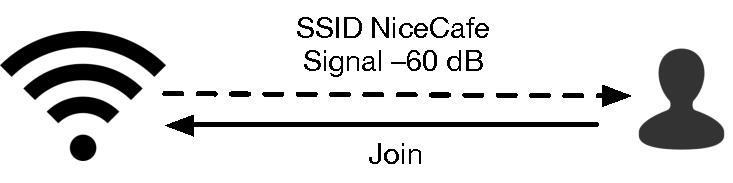
\includegraphics{images/evil_twin_normal.pdf}
      \label{subfig:evil_twin_normal}
    }
    \subfigure[Evil twin steals the connection with the same SSID]{
      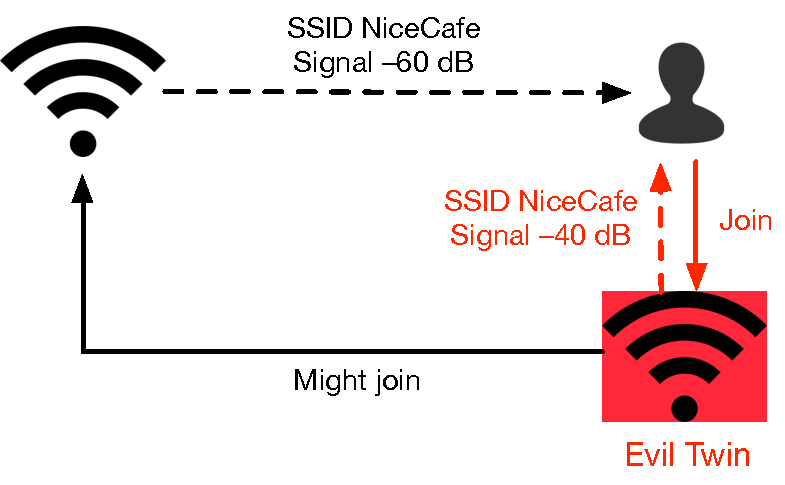
\includegraphics{images/evil_twin_mitm.pdf}
      \label{subfig:evil_twin_mitm}
    }
    \caption{Evil twin attack}
    \label{fig:evil_twin}
    \end{center}
\end{figure}

The idea of Evil twin attack is presented in Figure~\ref{fig:evil_twin}. First, there is a normal scenario. A user is having a coffee in his favorite cafe, and joins cafe's open network with an SSID \texttt{NiceCafe}. Everything goes well. The next time, the same user is visiting the cafe again, but this time there is an malicious access point with the same SSID, \texttt{NiceCafe}. Remember, SSID is not a unique identifier, and it can be chosen freely. The malicious one is located closer to the user or has more powerful antenna, so its signal is much stronger than the original AP's. Therefore, the user connects to malicious access point, and all the traffic is suddenly vulnerable.

\section{Man in the middle exploiting WLAN probes}

In previous section, an attacker knew beforehand that there was a specific network available and chose his SSID based on that. This is not necessary, and opens room for a more powerful attack.

A rogue access point can be listening for all the probes in the air. When it sees something, for example a node probing for a network \texttt{NiceCafe}, the AP can change its SSID to \texttt{NiceCafe} and let the node to connect.

If a node is not probing any specific SSID but asking all the nodes to broadcast theirs, the basic version of this attack will not obviously work. Still, there exists an opportunity: quite a many device has at one time connected to a network with an unchanged, manufacturer-default SSID, such as \texttt{Linksys} or \texttt{dlink}. According to Wigle \cite{wigle}, five most common SSIDs account for 4.2~\% of total SSIDs seen. An attacker could try all the common ones and hope that at least one of them is in node's SSID list.

\section{Encryption}

A particular problem for attackers is encryption. Wireless networks may be secured using techinques such as WPA2 (Wi-Fi Protected Access 2), which is based on pre-shared secret -- a passphrase. Since an attacker doesn't know the passphrase and it is not included in any probe requests, WPA2 renders this attack useless.

Another possible piece of encryption is Transport Layer Security, TLS (predecessor known as SSL, Secure Sockets Layer, and often these two are mixed). With a bit confusion with the name, it can be said that TLS is implemted between transport layer and application layer. As this layer is above link-layer, on which attacker operates, it should be a safe alternative.

However, there is a technique called sslstrip \cite{marlinspike2009new}, which is designed specifically to redirect badly-implemented TLS/SSL conenctions to unencrypted ones. At this time, using TLS can be considered only a partial solution against MITM attacks.

\section{Existing software and devices}

Concepts discussed here are not new, and for them there are specific tools implemented.

In previous section we mentioned technique called sslstrip; to prove its efficiency, authors decided to publish fully-working tool that implements the full attack. \cite{marlinspike2009new}

Most comprehensive and most easy-to-obtain toolkit is WiFi Pineapple \cite{wifipineapple}. It includes numerous tools for MITM and other attacks and sells for as low as \$~100 (as in August 2014).

With this kind of ready-made tools, performing man-in-the-middle attacks are totally feasible with only a little knowledge, and they must to be taken seriously.

%%%%%%%%%%%%%%%%%%%%%%%%%%%%%%%%%%%%%%%%%%%%%%%%%%%%%%%%%%%%%%%%%%%%%%%%%%%%%%%


\chapter{Legal status}
\label{chapter:legal}

is there any legislation? terms and conditions -- can't apply, if the user hasn't joined a network

approaches to get an ``I agree'' from customers: 
(1) put a physical sign (case Nordstrom, Inc) 
(2) use a specific app (case Helsinki-vantaa)
    -> if an app requires wifi permissions (on android), it can look easily for all previous networks (there was a paper on that)

\section{Europe}

\section{United States}


%%%%%%%%%%%%%%%%%%%%%%%%%%%%%%%%%%%%%%%%%%%%%%%%%%%%%%%%%%%%%%%%%%%%%%%%%%%%%%%


\chapter{Practical study}
\label{chapter:practical}

test in the wild, cover:

\section{Methodology}
\label{sec:methods}

\section{Commons}
\label{sec:practical_commons}

\section{Geolocation}
\label{sec:practical_geo}

\section{Semantic analysis}
\label{sec:practical_semantic}



%%%%%%%%%%%%%%%%%%%%%%%%%%%%%%%%%%%%%%%%%%%%%%%%%%%%%%%%%%%%%%%%%%%%%%%%%%%%%%%


\chapter{Countermeasures}
\label{chapter:countermeasures}

\section{Countermeasures for MAC address tracking}
apple randomize mac

ipv6 gives more address space in mac?


\section{Countermeasures for SSID profiling}
\label{sec:countermeasures_ssid}
broadcast

randomize mac for every probe request?

which one is more valuable, privacy or speed?

settings, defaults

modifying the protocol using cryptographic techniques~\cite{lindqvist2009privacy}

location-assisted: probe only networks nearby~\cite{kimposter}

\section{Securing against active attacks}

do not query for ssids

how about rogue AP guessing most used SSIDs?

save BSSID, ask for confirmation if SSID is the same, but BSSID is not? Windows Phone? 


%%%%%%%%%%%%%%%%%%%%%%%%%%%%%%%%%%%%%%%%%%%%%%%%%%%%%%%%%%%%%%%%%%%%%%%%%%%%%%%


\chapter{Conclusion}
\label{chapter:conclusion}


% Load the bibliographic references
% ------------------------------------------------------------------
% You can use several .bib files:
% \bibliography{thesis_sources,ietf_sources}
\bibliography{sources}


% Appendices go here
% ------------------------------------------------------------------
% If you do not have appendices, comment out the following lines
\appendix
\chapter{WPS Protocol}
\label{chapter:appendix:wps}

The full protocol for Wi-Fi Protected Setup (WPS) is presented on Figure~\ref{tab:wps_full} and is taken from~\cite{microsoftWCN}. Notations are as follows:

\textbf{E}: Enrollee

\textbf{R}: Registrar

\textbf{Mi}: Message $i$

\textbf{Mi*} Message $i$ without HMAC value

\textbf{N$_E$, N$_R$}: Nonces generated by enrollee and registrar

\textbf{PK$_E$, PK$_R$}: Enrollee's and registrar's public keys

\textbf{ConfigData}: WLAN settings and credentials

\textbf{AuthKey}: Key derived with Diffie-Hellman, using N$_E$, N$_R$, and enrollee's MAC address

\textbf{E-Hash1, E-Hash2, R-Hash1, R-Hash2}: Hashed device passwords, first and second half

\textbf{E-S1, E-S2, R-S1, R-S2}: Secret, encrypted nonces, that can be used with respective hashes (E-S1 $\leftrightarrow$ E-Hash1) to confirm the knowledge of device password

\begin{figure}
\label{tab:wps_full}
\begin{tabular}{c|c p{10cm}}

E $\rightarrow$ R & M1 = & Version $\|$ N$_E$ $\|$ Description $\|$ PK$_E$ 
\\\\

E $\leftarrow$  R & M2 = & Version $\|$ N$_E$ $\|$ N$_R$ $\|$ Description $\|$ PK$_R$ [ $\|$ ConfigData ] $\|$ HMAC$_{AuthKey}$(M1 $\|$ M2*) 
\\\\

E $\rightarrow$ R & M3 = & Version $\|$ N$_R$ $\|$ E-Hash1 $\|$ E-Hash2 $\|$ HMAC$_{AuthKey}$(M2 $\|$ M3*) 
\\\\

E $\leftarrow$  R & M4 = & Version $\|$ N$_E$ $\|$ R-Hash1 $\|$ R-Hash2 $\|$ ENC$_{KeyWrapKey}$(R-S1) $\|$ HMAC$_{AuthKey}$ (M3 $\|$ M4*) 
\\\\

E $\rightarrow$ R & M5 = & Version $\|$ N$_R$ $\|$ ENC$_{KeyWrapKey}$(E-S1) $\|$ HMAC$_{AuthKey}$ (M4 $\|$ M5*) 
\\\\

E $\leftarrow$  R & M6 = & Version $\|$ N$_E$ $\|$ ENC$_{KeyWrapKey}$(R-S2) $\|$ HMAC$_{AuthKey}$ (M5 $\|$ M6*) 
\\\\

E $\rightarrow$ R & M7 = & Version $\|$ N$_R$ $\|$ ENC$_{KeyWrapKey}$(E-S2 [$\|$ConfigData]) $\|$ HMAC$_{AuthKey}$ (M6 $\|$ M7*) 
\\\\

E $\leftarrow$  R & M8 = & Version $\|$ N$_E$ $\|$ [ENC$_{KeyWrapKey}$(ConfigData) ] $\|$ HMAC$_{AuthKey}$ (M7 $\|$ M8*) 
\\\\

\end{tabular}
\caption{Protocol for joining WPS-enabled WLAN. Modified from~\cite{microsoftWCN}}
\end{figure}


% End of document!
% ------------------------------------------------------------------
% The LastPage package automatically places a label on the last page.
% That works better than placing a label here manually, because the
% label might not go to the actual last page, if LaTeX needs to place
% floats (that is, figures, tables, and such) to the end of the 
% document.
\end{document}
